\section{Sistema propuesto}
Para este proyecto se planteó un sistema que implementa un control de FES en lazo cerrado utilizando la técnica de biofeedback. El sistema consiste en la adquisición de dos canales de sEMG, del brazo izquierdo, los cuales son procesados y se utilizan como entrada de un sistema de control que realiza la modulación de la amplitud de dos canales de estimulación eléctrica en el brazo derecho. Este sistema implementa un control contralateral para realizar un entrenamiento en espejo de las acciones de apertura y cierre de mano.

En la Figura \ref{Figura: SistProp} se muestra un esquema general del sistema desarrollado, en el cual se muestran en rojo los elementos implementados en este proyecto.

%Sistema propuesto
\begin{figure}[htbp]
\centering
	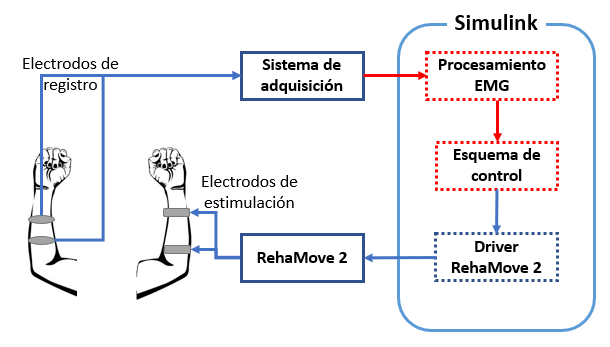
\includegraphics[scale=0.7]{SistemaPropuesto.png}
	\caption[Sistema propuesto para el proyecto]{Sistema propuesto para el proyecto. Líneas continuas representan entes de hardwares y líneas discontinuas representan entes de software. Elementos en rojo representan zonas de trabajo del proyecto.}
	\label{Figura: SistProp}
\end{figure}


\section{Adquisición de datos en Simulink\textregistered} \label{Sec: Adquisicion}
Para realizar la adquisición de las señales de sEMG se utilizó el sistema Cyton Board, el cual tiene una frecuencia de muestreo de 250 Hz. Dicho sistema utiliza un chip ADS1299 (Texas Instruments Inc., Dallas, E.U.A.) para realizar la conversión analógico-digital de las señales, el cual codifica los datos de cada muestra, utilizando codificación en complemento a 2, en un flujo de datos de 27 bytes en formato MSBF (most significant bit first) esquematizado en la Figura \ref{Figura: BusOut}. En dicha figura se aprecia claramente que cada muestra de cada canal está conformada por 3 bytes , formando un total de 24 bytes para los 8 canales, mientras que los primeros 3 bytes corresponden a información de estado propia del ADS1299.

%Stream datos ADS
\begin{figure}[htbp]
\centering
	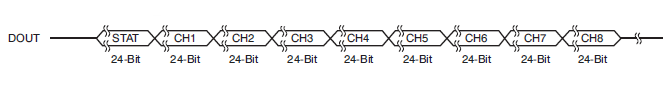
\includegraphics[scale=0.8]{Bus_Dat_Out_ADS.png}
	\caption{Flujo de datos de salida del ADS1299.}
	\label{Figura: BusOut}
\end{figure}

Para realizar la decodificación del flujo de datos dentro de Simulink\textregistered, se diseñó un subsistema encargado de la solicitud y decodificación de datos, para esto se utilizó el bloque \emph{Query Instrument} del \emph{Instrument Control Toolbox} para realizar la solicitud de datos, los cuales fueron decodificados con bloques de la librería estándar de Simulink\textregistered. La figura \ref{Figura: DecoSimuT} muestra la implementación de este subsistema.

%\hfill \break
\vfill
%Sistema Simulink
\begin{figure}[htbp]
	\centering
	\begin{subfigure}[htbp]{0.8\textwidth}
		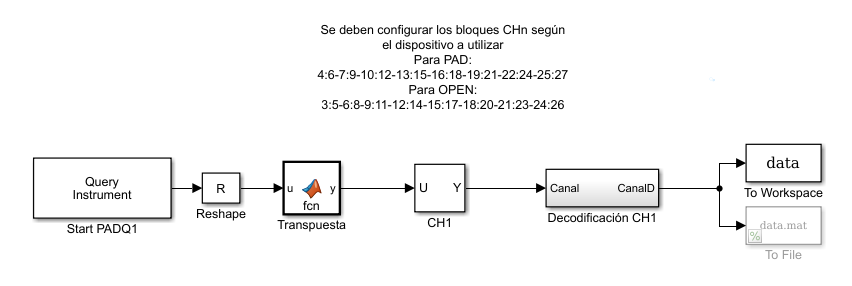
\includegraphics[width=\textwidth]{Read_Simu.png}
		\caption{}
		\label{Figura: readSimu}
	\end{subfigure}
	\begin{subfigure}[htbp]{0.75\textwidth}
		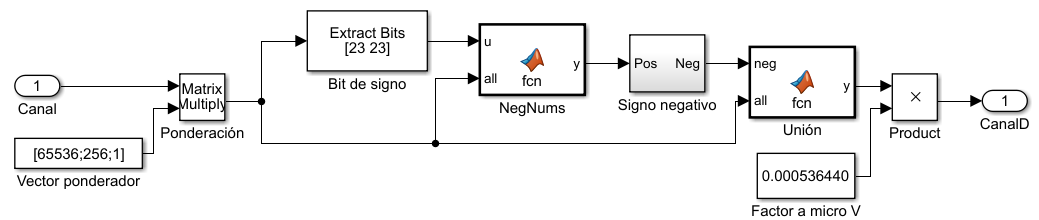
\includegraphics[width=\textwidth]{Deco_Simu.png}
		\caption{}
		\label{Figura: decoSimu}
	\end{subfigure}
	\caption[Diagrama de bloques del subsistema decodificador del flujo de datos]{Diagrama de bloques del subsistema decodificador del flujo de datos implementado en Simulink\textregistered . (a) Vista general del subsistema diseñado para realizar adquisición y decodificación del flujo de datos. (b) Vista interna del subsistema encargado de la decodificación del flujo de datos.}
	\label{Figura: DecoSimuT}
\end{figure}

\newpage
El funcionamiento del subsistema responsable de la solicitud y decodificación de datos implementado dentro de Simulink\textregistered \; se encuentra esquematizado en la Figura \ref{Figura: DecoStream}, y lleva a cabo el siguiente algoritmo:

\begin{enumerate}
	\item Se realiza la adquisición de N muestras, lo cual generará un vector columna con dimensión $(27*N)\times 1$ (Figura \ref{Figura: DecoStream} \emph{(a)}), donde 27 corresponde al tamaño en bytes del flujo de datos a recibir y 1 corresponde a 1 columna en la que se recibirán los datos. %$\mathbb{R}^{27*N\times 1}$
	
	\item Se aplica una operación de reshape a dicho vector para obtener una matriz con dimensión $27\times N$ (Figura \ref{Figura: DecoStream} \emph{(b)}). %$\mathbb{R}^{27\times N}$
	
	\item Se obtiene la transpuesta de dicha matriz para obtener una matriz de dimension $N\times 27$ (Figura \ref{Figura: DecoStream} \emph{(c)}). %$\mathbb{R}^{N\times 27}$
	
	\item Se realiza la extracción de las columnas asociadas al canal a procesar, obteniendo una matriz de dimensión $N\times 3$ (Figura \ref{Figura: DecoStream} \emph{(d)}), donde 3 es el número de bytes correspondientes a cada muestra. %$\mathbb{R}^{N\times 3}$
	
	\item Se realiza el producto de la matriz del canal a procesar con un vector (columna) ponderador que contiene el peso de cada columna (byte) necesario para obtener el valor de la muestra de 24 bits (Figura \ref{Figura: DecoStream} \emph{(e)}). El vector ponderador está compuesto por los valores $2^{16}$, $2^8$ y $2^0$, los cuales corresponden a realizar un corrimiento hacia la izquierda de 16, 8 y 0 bits respectivamente. Como resultado de dicho producto se obtiene un vector de dimensión $N\times 1$ en unidades de bits (Figura \ref{Figura: DecoStream} \emph{(f)}). %$\mathbb{R}^{N\times 1}$
	
	\item Se extraen del vector \emph{f} las muestras en las que se encuentren codificados, en complemento a 2, un número negativo. Esto se realiza al obtener el valor del bit 23 (bit más significativo), y si dicho bit tiene un valor de 1 implica que dicha muestra codifica un número negativo. De esta operación se obtiene un vector con dimensión $M\times 1$, donde $M$ es la cantidad de muestras negativas a decodificar. (Figura \ref{Figura: DecoStream} \emph{(g)}).
	
	\item Se obtiene el complemento a 1 de cada elementro (muestra) del vector \emph{g}, sumando 1 a cada muestra y multiplicándola por -1. De esta operación se obtiene un vector con las muestras decodificadas a número binarios con signo negativo (Figura \ref{Figura: DecoStream} \emph{(h)}).
	
	\item Se insertan los elementos del vector \emph{h} en sus posiciones originales del vector \emph{f}. De este último paso se obtiene un vector con las N muestras decodificadas a números de 24 bits con signo en unidades de bits (Figura \ref{Figura: DecoStream} \emph{(i)}).
	
	\item Por último, para  obtener unidades de voltaje, se multiplica cada elemento del vector \emph{i} por un factor de escalamiento determinado por la Ecuación \ref{Ecu: ScaleFactor}. Obteniendo como resultado un vector columna con las N muestras adquiridas en unidades de voltaje.
\end{enumerate}

\vfill
\begin{equation}
	Factor\; de\; Escalamiento = V_{ref}/(2^{23}-1)/Ganancia
	\label{Ecu: ScaleFactor}
\end{equation}
\vfill
%Funcionamiento decodificación
\begin{figure}[htbb]
\centering
	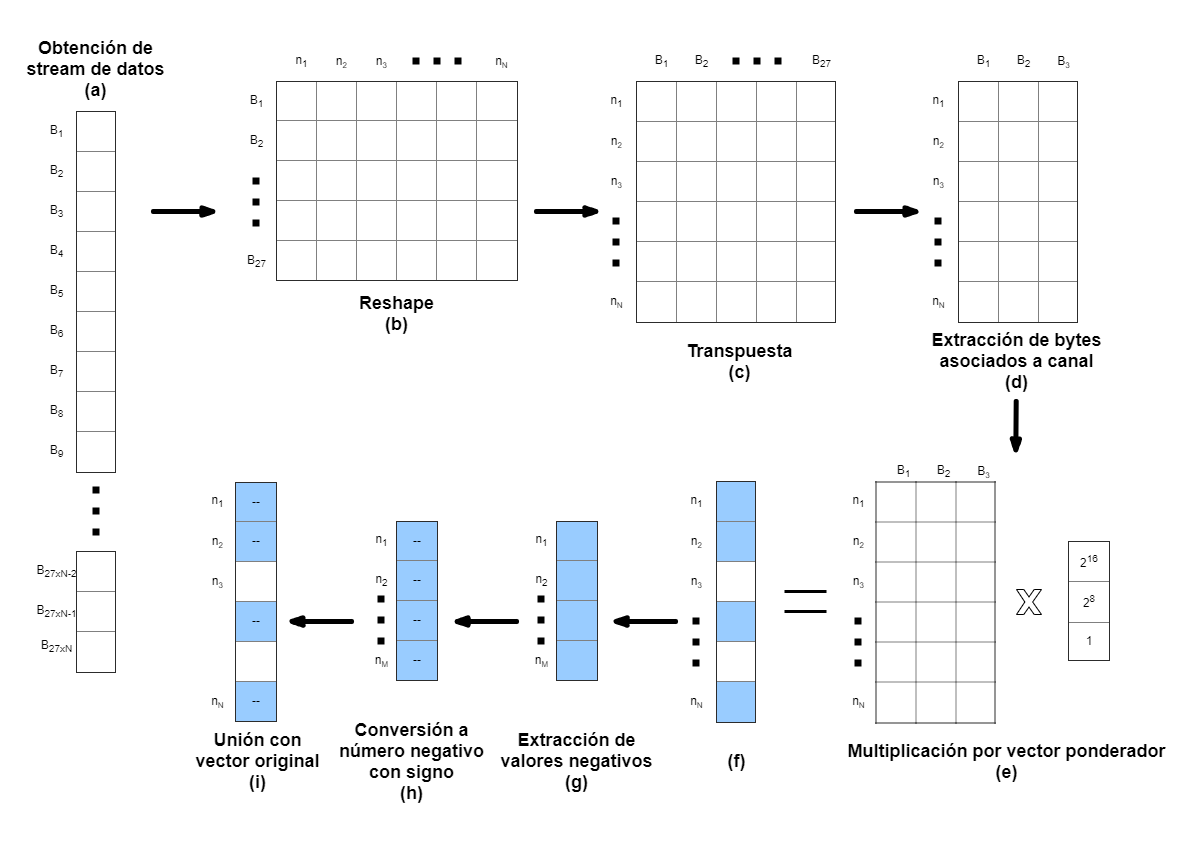
\includegraphics[width=\textwidth]{DecoStream.png}
	\caption{Funcionamiento del subsistema decodificador del flujo de datos.}
	\label{Figura: DecoStream}
\end{figure}
\vfill

\newpage
\section{Evaluación de bloque de adquisición y decodificación}\label{Sec: EvalAdquisicion}
Se llevó a cabo un procedimiento para evaluar el desempeño del subsistema diseñado en Simulink\textregistered \; para la adquisición y decodificación de datos. En MATLAB\textregistered \; se generó un banco de señales senoidales conformado por 5 senoidales puras de 1 Hz, 5 Hz, 10 Hz, 20 Hz, 50 Hz y 100 Hz (Figura \ref{Figura: SenPur}), tres senoidales de 50 Hz moduladas en amplitud con distintas envolventes: 
una envolvente de una recta con pendiente negativa (Figura \ref{Figura: LinAte}), una envolvente de una exponencial decreciente (Figura \ref{Figura: ExpAte}), y una envolvente que simula la señal sEMG correspondiente a la tarea de incrementar gradualmente una contracción muscular, mantener dicha contracción y relajar el músculo gradualmente (Figura \ref{Figura: Contra}). Todas las señales del banco se diseñaron con una frecuencia de muestreo de 250 Hz y una duración de 5 segundos, excepto la última, que se diseñó con una duración de 15 segundos; adicionalmente, todas las señales se generaron como objetos de audio dentro de MATLAB\textregistered, para poder reproducirlas como audio y a partir de la salida de audio de la computadora poder acceder a ellas.

%Figura de senoidales MATLAB
\begin{figure}[htbp]
	\centering
	\begin{subfigure}[htbp]{0.45\textwidth}
		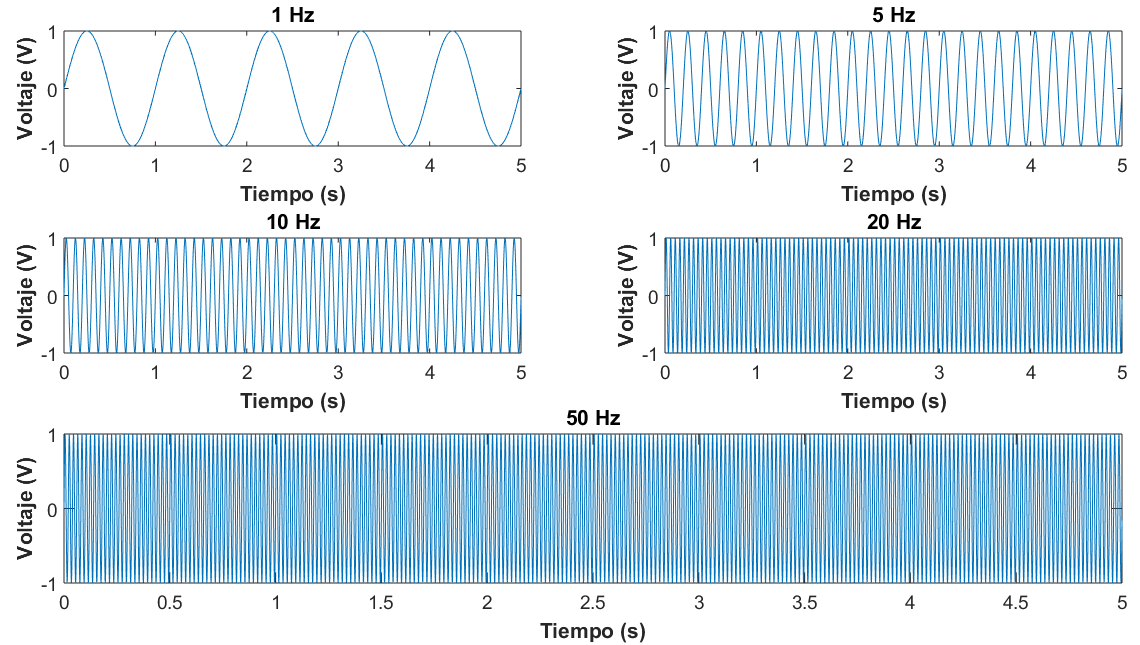
\includegraphics[width=\textwidth]{Sen_Pur.png}
		\caption{}
		\label{Figura: SenPur}
	\end{subfigure}
	\hfill
	\begin{subfigure}[htbp]{0.45\textwidth}
		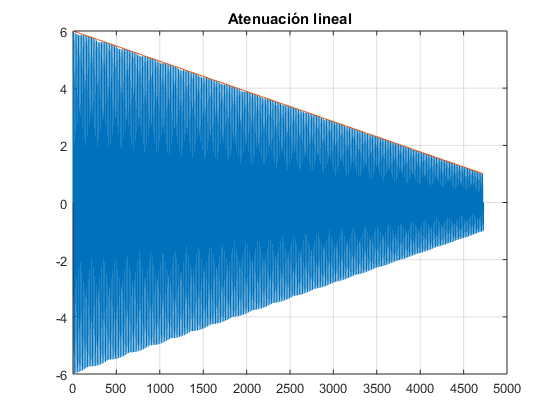
\includegraphics[width=\textwidth]{Lin_Ate.png}
		\caption{}
		\label{Figura: LinAte}
	\end{subfigure}
	\hfill
	\begin{subfigure}[htbp]{0.45\textwidth}
		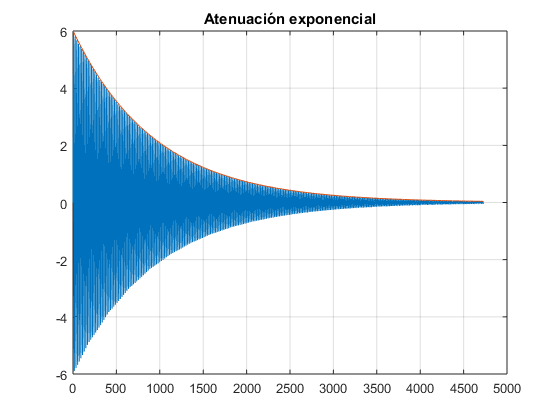
\includegraphics[width=\textwidth]{Exp_Ate.png}
		\caption{}
		\label{Figura: ExpAte}
	\end{subfigure}
	\hfill
	\begin{subfigure}[htbp]{0.45\textwidth}
		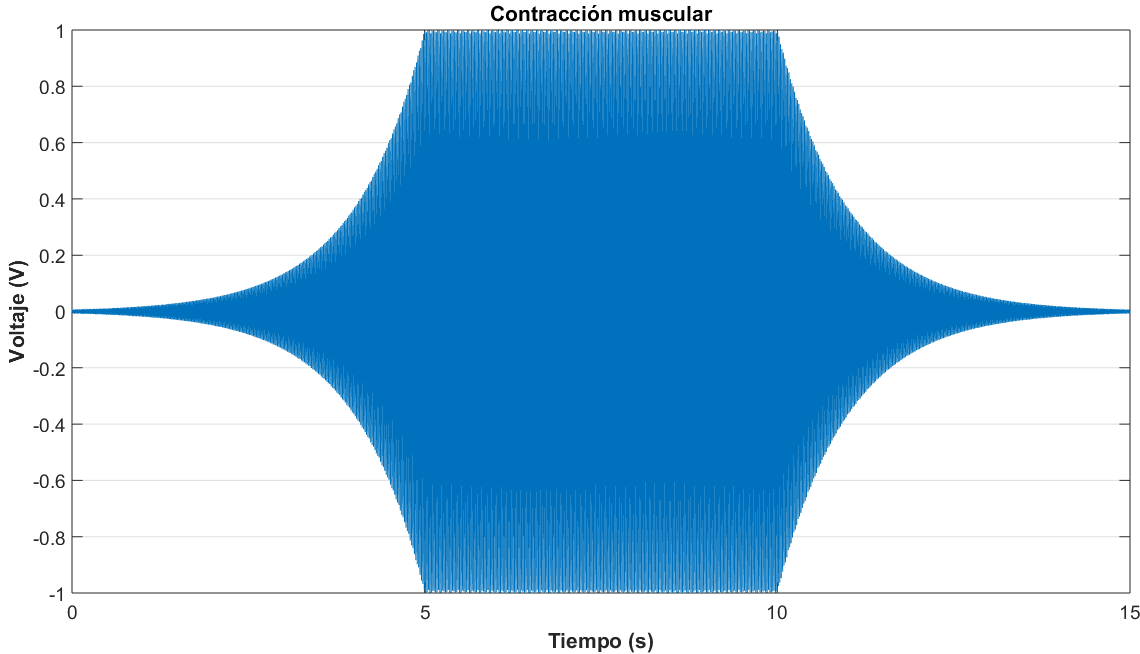
\includegraphics[width=\textwidth]{Contra.png}
		\caption{}
		\label{Figura: Contra}
	\end{subfigure}	
	\caption[Banco de señales para evaluación de adquisición]{Banco de señales para evaluación de adquisición. (a) Senoidales puras a diferentes frecuencias. (b) Senoidal de 50 Hz con atenuación lineal. (c) Senoidal de 50 Hz con atenuación exponencial. (d) Senoidal de 50 Hz simulando el sEMG de una contracción muscular.}
	\label{Figura: SenalesEva}
\end{figure}

\newpage
El proceso para la evaluación del funcionamiento del subsistema de adquisición se llevó a cabo de la siguiente manera:
\begin{enumerate}
	\item Se realiza la adquisición de tres repeticiones de cada una de las señales del banco de señales de prueba.
	\begin{enumerate}
		\item Se conecta una punta de un jack de audio de 3.5 mm a la salida de audio de la computadora. La otra punta se conectó al dispositivo de adquisición (Cyton Board) de la siguiente forma: el pin \emph{izquierdo} se conectó a un pin diferencial del canal 1, mientras que el pin \emph{tierra} se conectó a la entrada BIAS y al pin diferencial restante del canal 1. La Figura \ref{Figura: JackConexion} ilustra estas conexiones.
		\item Se realiza la solicitud de datos utilizando el subsistema decodificador implementado en Simulink\textregistered \; (Figura \ref{Figura: DecoSimuT}), y al mismo tiempo se inicia el conteo de un cronómetro.
		\item Dos segundos después de haber iniciado la solicitud de datos, se procede a reproducir la señal de audio de prueba.
		\item Tras haber transcurrido 10 s (20 s para la simulación del sEMG de una contracción), se detiene la adquisición del subsistema de Simulink\textregistered \; y se guardan los datos registrados dentro de un archivo con extensión \emph{.mat}.
	\end{enumerate}
	\item Se cargan, dentro del workspace de MATLAB\textregistered, los datos de las señales adquiridas y los datos de las señales patrón.
	\item Se procede a alinear de forma manual la señal adquirida con la señal patrón, y posteriormente se calcula el coeficiente de correlación de Pearson (Ecuación \ref{Ecu: CorrePea}. Donde $\sigma_{xy}$ representa la covarianza de $x$,$y$; $\sigma_{x}$ representa la desviación estándar de $x$; y $\sigma_{y}$ representa la desviación estándar de $y$) entre ambas señales.
	\item Se obtiene la media aritmética de los valores obtenidos al aplicar el coeficiente de correlación de Pearson a cada una de las señales registradas (24 registros en total). El valor obtenido se utiliza como indicador de la calidad del subsistema de adquisición y decodificación de datos.
\end{enumerate}

\vfill
%Ecuación correlación Pearson
\begin{equation}
	r = \frac{\sigma_{xy}}{\sigma_{x}\sigma_{y}}
	\label{Ecu: CorrePea}
\end{equation}
\vfill

\begin{figure}
	\centering
	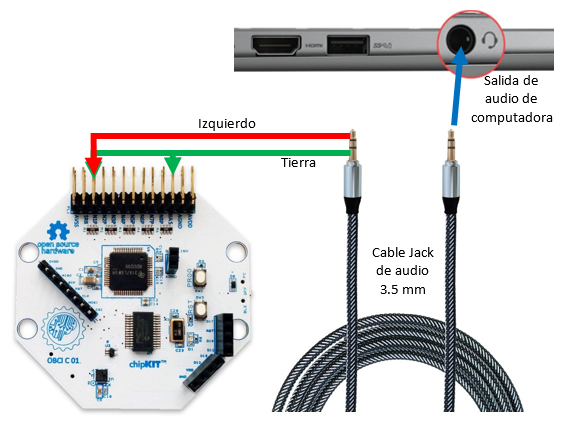
\includegraphics[width=0.5\textwidth]{JackConexion.png}
	\caption{Conexiones para evaluación de bloque de adquisición.}
	\label{Figura: JackConexion}
\end{figure}

\newpage
\section{Protocolo para registro de sEMG}\label{Sec: ProReg}
Para garantizar repetibilidad en los registros de sEMG se implementó un protocolo para realizar la adquisición de dicha señal. Dicho protocolo se describe a continuación y utiliza electrodos Telectrode T718 (Bio-Protech Inc., Chino, E.U.A.):

\begin{enumerate}
	\item Se configura el dispositivo de adquisición (Para el caso del Cyton Board esta configuración es la preprogramada por el fabricante):
	\begin{enumerate}
		\item Frecuencia de muestreo a 250 Hz.
		\item Ganancia 24 para los canales de adquisición 1 y 2.
		\item BIAS (función de reducción de ruido común) habilitado para los canales de adquisición 1 y 2.
	\end{enumerate}
	\item Se preparan las zonas donde se colocaran los electrodos para registro de sEMG, limpiando con algodón y alcohol las zonas ventral y dorsal del antebrazo, así como el codo.
	\item Se ubican los puntos para colocación de electrodos:
	\begin{enumerate}
		\item Para el par de electrodos que registrará la actividad relacionada con el movimiento de flexión de dedos (pinza gruesa), el músculo asociado es el músculo flexor digitorum (Figura \ref{Figura: E_Cie}):
		\begin{enumerate}
			\item Se mide la distancia de codo a muñeca en el lado ventral del antebrazo.
			\item Se coloca una marca al 25\% de la medida obtenida.
		\end{enumerate}
		\item Para el par de electrodos que registrará la actividad relacionada con el movimiento de extensión de dedos (apertura de mano), el músculo asociado es el músculo extensor digitorum (Figura \ref{Figura: E_Ape}):
		\begin{enumerate}
			\item Se mide la distancia de codo a muñeca en el lado dorsal del antebrazo.
			\item Se coloca una marca al 75\% de la medida obtenida.
		\end{enumerate}
	\end{enumerate}
	\item Se colocan, centrados sobre la marca obtenida para el flexor digitorum (Figura \ref{Figura: E_Cie}), dos electrodos (en dirección de las fibras musculares) separados 3 cm. Este par de electrodos se conecta al canal 1 del dispositivo de adquisición por medio de cables con conector tipo Snap.
	\item Se colocan, centrados sobre la marca obtenida para el extensor digitorum (Figura \ref{Figura: E_Ape}), dos electrodos (en dirección de las fibras musculares) separados 3 cm. Este para de electrodos se conecta al canal 2 del dispositivo de adquisición por medio de cables con conector tipo Snap.
	\item Se coloca un electrodo de referencia sobre el codo. Dicho electrodo se conecta al pin BIAS del dispositivo de adquisición.
\end{enumerate}

\vfill
%Ubicación electrodos
\begin{figure}[htbp]
	\centering
	\begin{subfigure}[htbp]{0.3\textwidth}
		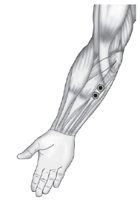
\includegraphics[width=\textwidth]{E_Cie.png}
		\caption{}
		\label{Figura: E_Cie}
	\end{subfigure}
%	\hfill
	\hspace{3cm}
	\begin{subfigure}[htbp]{0.3\textwidth}
		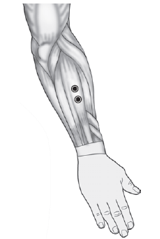
\includegraphics[width=\textwidth]{E_Ape.png}
		\caption{}
		\label{Figura: E_Ape}
	\end{subfigure}
	\caption[Posicionamiento de electrodos para registro de sEMG]{Posicionamiento de electrodos para registro de sEMG. Adaptado de \cite{Cavalcanti-Garcia2009}. (a) Ubicación de electrodos para flexor digitorum. (b) Ubicación de electrodos para extensor digitorum.}
	\label{Figura: E_sEMG}
\end{figure}
\vfill

\newpage
\section{Procesamiento de sEMG} \label{Sec: Procesamiento}
Se diseñaron tres filtros digitales Butterworth de orden 2 para realizar el procesamiento de sEMG:

\begin{itemize}
	\item Un filtro pasa altas con frecuencia de corte de 15 Hz, para eliminar las variaciones en la línea base del registro.
	\item Un filtro pasa bajas con frecuencia de corte de 100 Hz, para eliminar armónicos de 60 Hz y demás interferencias de alta frecuencia.
	\item Un filtro rechaza banda centrado en 60 Hz, para reducir la interferencia de la línea
\end{itemize}

Todos estos filtros se diseñaron utilizando la función \emph{butter} de MATLAB\textregistered. Las gráficas de respuesta en frecuencia de estos filtros se muestran en la Figura \ref{Figura: Freqz_Filtros} %las Figuras \ref{Figura: FiltroPA} a \ref{Figura: FiltroRB}.

%Respuesta en frecuencia de filtros
\begin{figure}[htbp]
	\centering
	\begin{subfigure}[htbp]{0.7\textwidth}
		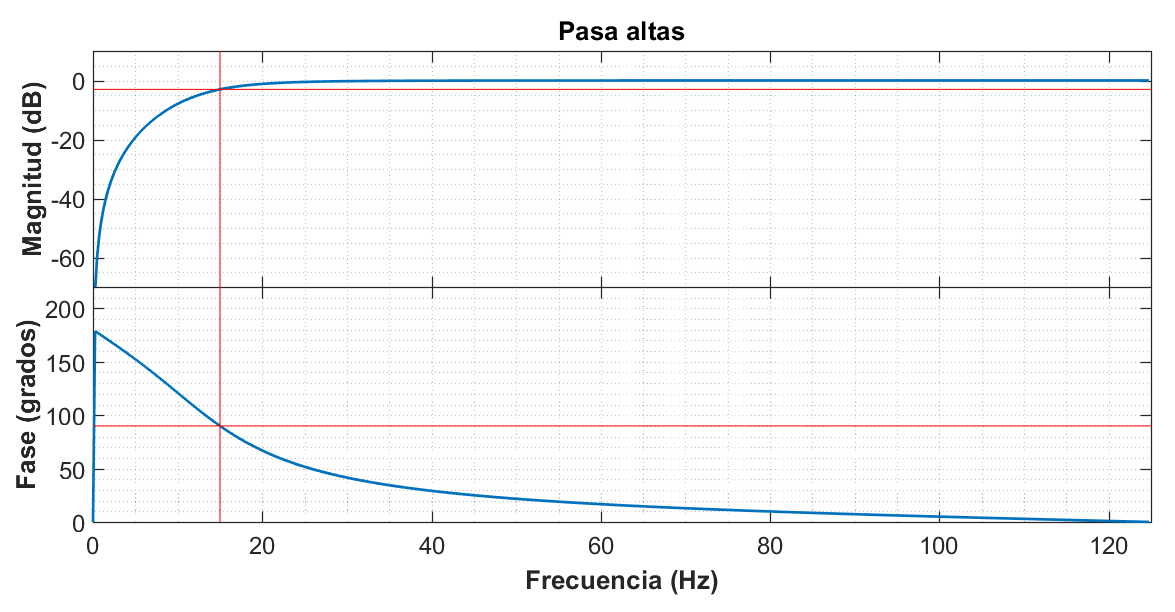
\includegraphics[width=\textwidth]{FiltroPA15Hz_PADQ.png}
		\caption{}
		\label{Figura: FiltroPA}
	\end{subfigure}
	
	\begin{subfigure}[htnp]{0.7\textwidth}
		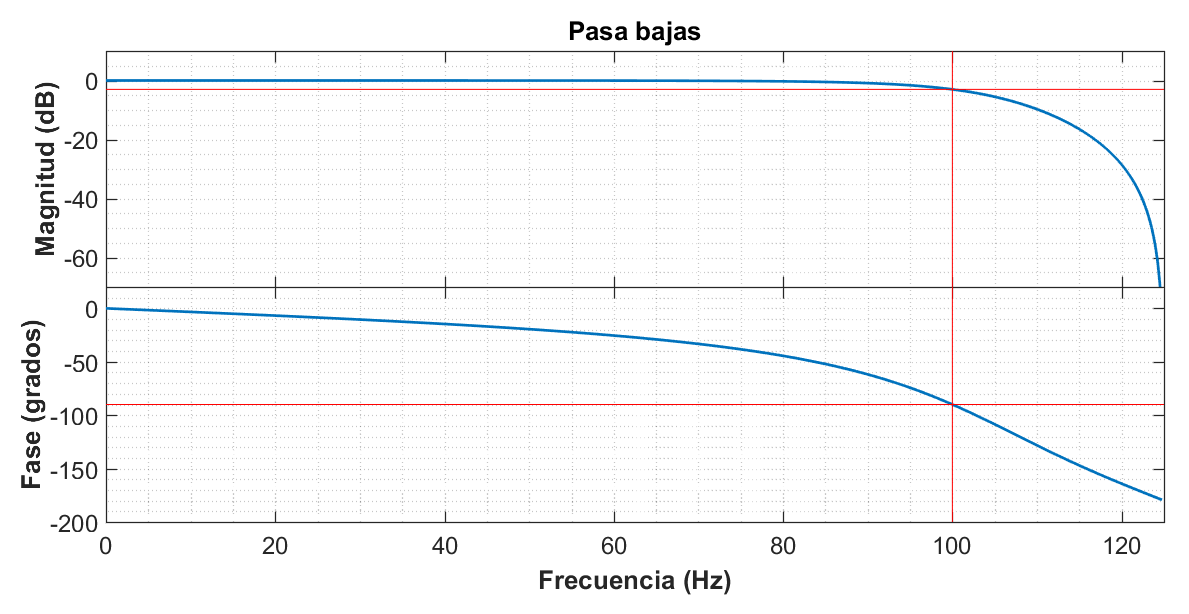
\includegraphics[width=\textwidth]{FiltroPB100Hz_PADQ.png}
		\caption{}
		\label{Figura: FiltroPB}
	\end{subfigure}
	
	\begin{subfigure}[htbp]{0.7\textwidth}
		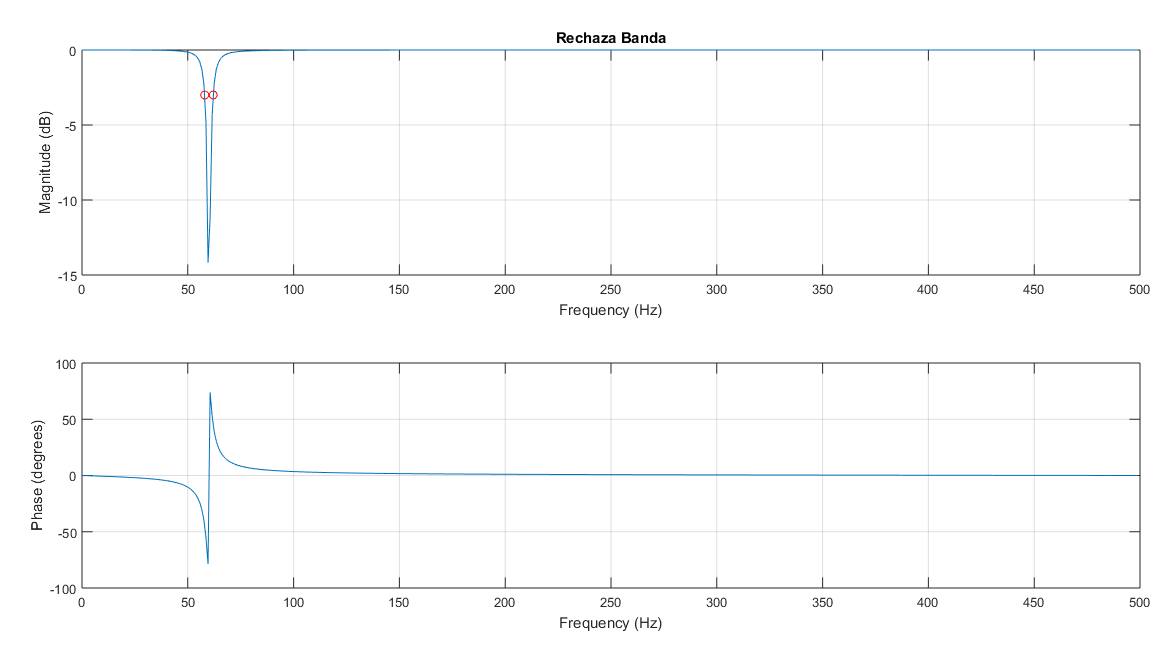
\includegraphics[width=\textwidth]{FiltroRB_58_62_PADQ.png}
		\caption{}
		\label{Figura: FiltroRB}
	\end{subfigure}
	\caption[Respuesta en frecuencia del banco de filtros diseñado]{Respuesta en frecuencia del banco de filtros diseñado. (a) Filtro pasa altas. (b) Filtro pasa bajas. (c) Filtro rechaza banda.}
	\label{Figura: Freqz_Filtros}
\end{figure}

Se implementó dentro de Simulink\textregistered \;un bloque responsable de obtener el valor RMS de ventanas de 100 ms (25 muestras para una frecuencia de muestro de 250 Hz) del registro de sEMG, para utilizar dicho descriptor de amplitud como señal de control. Adicionalmente se implementó un filtro de mediana de 10 muestras (Ecuación \ref{Ecu: Mediana}), el cual tiene como propósito conseguir una señal RMS suavizada.

%Ecuación filtro mediana
\begin{equation}
	y[n] = mediana(x[n]:x[n-N])
	\label{Ecu: Mediana}
\end{equation}


\newpage
\section{Sistema de control}
A grandes rasgos, el sistema de control implementado para este proyecto consta de la combinación de una FSM y un mapeo proporcional. La FSM (Figura \ref{Figura: FSM_Control})  determina el canal de estimulación eléctrica que se activará, a partir de la salida del algoritmo para la detección de movimiento, el cual clasifica la intención de movimiento del sujeto en tres clases (descanso, pinza gruesa y apertura de mano), mientras que el mapeo proporcional permite realizar la modulación de la amplitud de corriente eléctrica a partir de la amplitud del sEMG.

%permite clasificar la intención de movimiento del sujeto en tres clases (descanso, pinza gruesa y apertura de mano), mientras que el control proporcional permite realizar la modulación de la amplitud de corriente eléctrica a partir de la amplitud del sEMG.

%FSM
\begin{figure}[htbp]
	\centering
	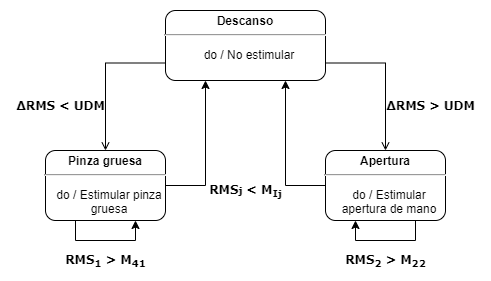
\includegraphics[scale=0.7]{FSM_Control.png}
	\caption[FSM para control]{Máquina de estados finitos encargada de la detección de movimiento e inicio del control proporcional.}
	\label{Figura: FSM_Control}
\end{figure}

La máquina de estados necesita principalmente tres parámetros para llevar a cabo la transición entre los movimientos: umbral detector de movimiento ($UDM$), umbral de pinza gruesa incompleta ($M_{1I}$) y umbral de apertura de mano incompleta ($M_{2I}$), y dentro de los estados pinza gruesa y apertura, la FSM necesita de la ecuación de mapeo proporcional para poder llevar a cabo la modulación de la estimulación eléctrica. La obtención de dichos parámetros se obtiene de un proceso de calibración que se realiza para cada sesión de prueba.

Posterior al proceso de calibración se realiza una validación fuera de línea, donde a partir del registro de calibración y los parámetros arrojados por esta se pone a prueba el funcionamiento del sistema. Cuando la validación fuera de línea presenta un porcentaje de acierto igual o mayor al 80$\%$ se procede a configurar el sistema para realizar una prueba en línea y posteriormente realizar la tarea objetivo.

Todas las etapas antes mencionadas del sistema de control se describen a continuación.

\subsection{Calibración}\label{Sec: Calibracion}
El proceso de calibración del sistema se divide en una calibración de los parámetros de estimulación eléctrica y una calibración de los valores de amplitud RMS del sEMG.

\subsubsection{Calibración de parámetros FES}\label{Sec:CalFES}
El objetivo de esta calibración es el obtener los umbrales motores y funcionales de los movimientos de apertura de mano y pinza gruesa. Para esta calibración se utiliza el sistema de colocación de electrodos de estimulación eléctrica desarrollado en el INR-LGII, el cual se encuentra descrito en \cite{AnaMartin2019}, en conjunto con la pantalla \emph{Experimentación} (Figura \ref{Figura: GUI_Exp}) de la GUI diseñada en el INR-LGII \cite{JanethFuentes2018}.

El proceso para la obtención de los umbrales antes mencionados consiste en realizar la colocación de los electrodos de estimulación eléctrica y realizar una exploración de la respuesta del sujeto ante diferentes valores de amplitud de corriente eléctrica que le serán proporcionados. Dichos valores exploran el rango entre 1 y 15 mA, utilizando un incremento de 1 mA. El umbral motor será el primer valor de amplitud que genere una respuesta motora notable a simple vista y reconocida por el sujeto en la mano del sujeto; mientras que el umbral funcional será aquél valor de amplitud que provoque el movimiento objetivo de la mano con un rango de movimiento completo, similar a un movimiento voluntario

%Experimentación
\begin{figure}[htb]
	\centering
	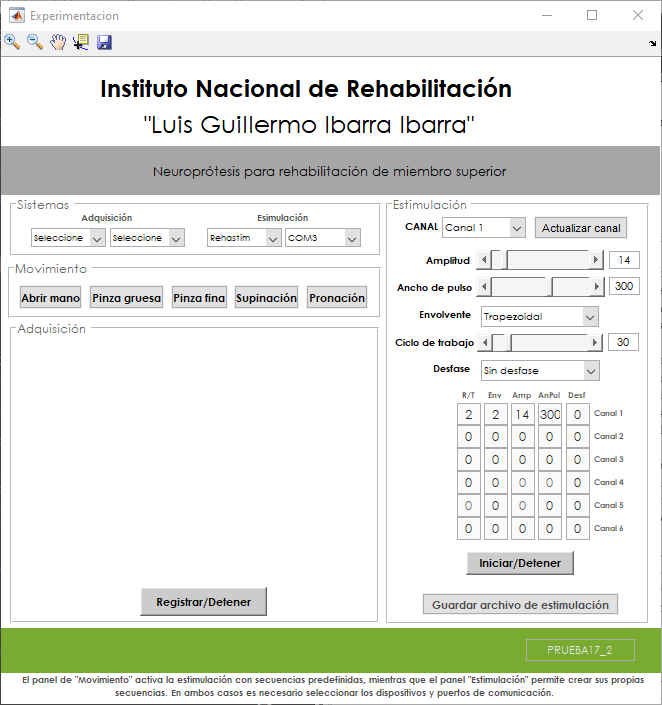
\includegraphics[width=0.6\textwidth]{GUI_Exp.png}
	\caption{GUI utilizada para calibración de FES.}
	\label{Figura: GUI_Exp}
\end{figure}

\subsubsection{Calibración de umbrales RMS de sEMG}\label{Sec:CalRMS}
Para realizar esta calibración se utiliza el protocolo de registro descrito en la sección \ref{Sec: ProReg} y una pantalla de calibración diseñada para este proyecto (Figura \ref{Figura: GUI_Ent}), la cual muestra indicaciones en forma de texto de los movimientos que debe realizar el sujeto y a la par realiza el registro de sEMG y almacena marcadores asociados a la indicación de movimiento solicitada. Una vez colocados los electrodos para registro de sEMG, se le muestra al sujeto cuales son los movimientos asociados a cada una de las indicaciones que se le irán mostrando en la GUI. Los movimientos mostrados son denominados \emph{descanso} (DD), \emph{apertura incompleta} (AI), \emph{apertura completa} (AC), \emph{pinza gruesa incompleta} (CI) y \emph{pinza gruesa completa} (CC), los cuales se pueden observar en la Figura \ref{Figura: Posturas}.

Al terminar las repeticiones de los movimientos solicitados, la GUI nos arroja en la consola de MATLAB\textregistered \; los valores de los umbrales RMS para los movimientos apertura de mano incompleta y completa (ambos relacionados al canal 2 de registro y estimulación), pinza gruesa incompleta y completa (ambos relacionados al canal 1 de registro y estimulación), y descanso, para cada canal de registro. La obtención de estos umbrales se realiza mediante la Ecuación \ref{Ecu: U_RMS}, donde $M_{ij}$ representa el umbral del i-ésimo movimiento registrado en el j-ésimo canal, $RMS_n$ representa al valor RMS obtenido para la n-ésima ventana de registro (100 ms) asociada al movimiento $M_{ij}$, y $N$ representa la cantidad de valores RMS asociados al movimiento $M_{ij}$.

%donde $M_i$ representa a uno de los 5 movimientos antes mencionados, $RMS_n$ representa al valor RMS obtenido para la n-ésima ventana de registro (100 ms) asociada al movimiento $M_i$, y $N$ representa la cantidad de valores RMS asociados al movimiento $M_i$.

%Ecuación obtención de umbrales
\begin{equation}
	M_{ij} = \frac{\sum_{n=1}^{N}RMS_{n}}{N}
	\label{Ecu: U_RMS}
\end{equation}

La GUI también proporciona un valor denominado \emph{umbral de detección de movimiento} (UDM), y los parámetros de las rectas que se utilizarán para llevar a cabo el control lineal.

El UDM, junto a los umbrales de movimiento incompleto, se utilizan para determinar la transición de estados de la FSM, siendo esta la encargada de activar el canal de estimulación eléctrica asociado a la intención de movimiento del sujeto. El UDM se obtiene utilizando la Ecuación \ref{Ecua: DM}, donde $RMS_{2n}$ y $RMS_{1n}$ representan el valor RMS de la n-esima ventana de registro para el movimiento de apertura incompleta en los canales 2 y 1 respectivamente, y $N$ representa la cantidad de valores RMS existentes para el movimiento de apertura incompleta.

%Ecuación detector movimiento
\begin{equation}
	UDM = \frac{\sum_{n=1}^{N}RMS_{2n}-RMS_{1n}}{N}
	\label{Ecua: DM}
\end{equation}

Los parámetros de las rectas que arroja la GUI son la pendiente (m) y la ordenada al origen (b), donde dichas rectas son utilizadas para llevar a cabo el mapeo proporcional de los movimientos apertura de mano y pinza gruesa. Estos parámetros se obtienen a partir de las Ecuaciones \ref{Ecu: m} y \ref{Ecu: b}, donde $m_{j}$ y $b_{j}$ representan la pendiente y ordenada al origen, respectivamente, de la j-ésima recta correspondiente al j-ésimo canal de estimulación; $U_{Fj}$ y $U_{Mj}$ representan los umbrales funcionales y motores, respectivamente, obtenidos tras la calibración de parámetros FES para el j-ésimo movimiento correspondiente; $M_{Cj}$ y $M_{Ij}$ representan los umbrales de los movimientos completos e incompletos, respectivamente, del j-ésimo canal de registro. Una vez determinados estos parámetros, se tienen todos los elementos necesarios para probar y usar el sistema sEMG-FES.

\vfill
%Ecuación pendiente
\begin{equation}
	m_{j} = \frac{ U_{jF} - U_{jM} }{ M_{Cj} - M_{Ij} }
	\label{Ecu: m}
\end{equation}

\vfill
%Ecuación ordenada
\begin{equation}
	b_{j} = U_{jM} - m_{j}*M_{Ij}
	\label{Ecu: b}
\end{equation}

\vfill
%Entrenamiento_sEMG
\begin{figure}[htb]
	\centering
	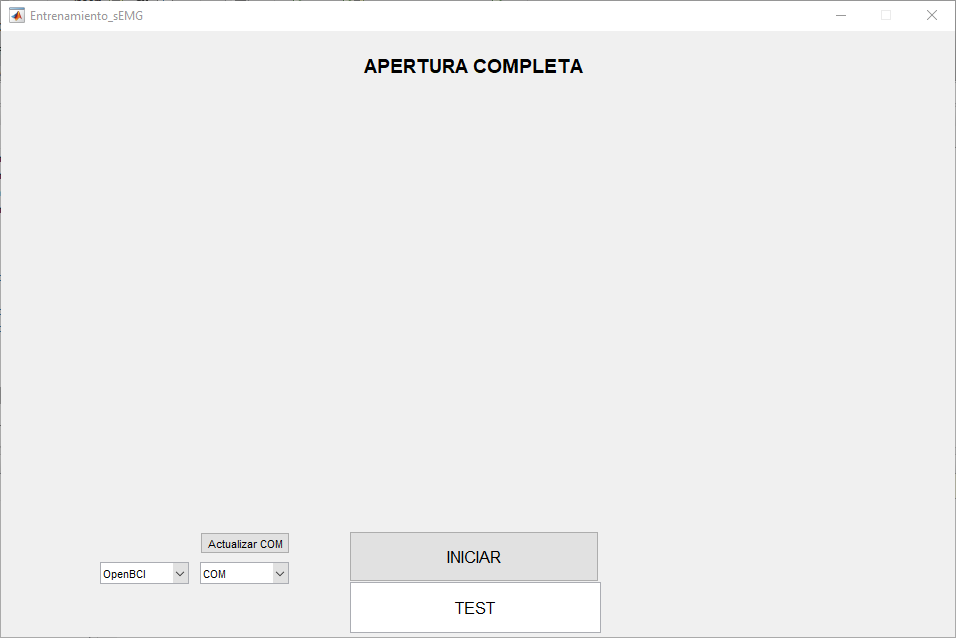
\includegraphics[width=0.7\textwidth]{GUI_Ent.png}
	\caption{GUI utilizada para calibración de amplitud RMS.}
	\label{Figura: GUI_Ent}
\end{figure}

%Posturas manos
\begin{figure}[htbp]
	\centering
	\begin{subfigure}[htbp]{0.4\textwidth}
		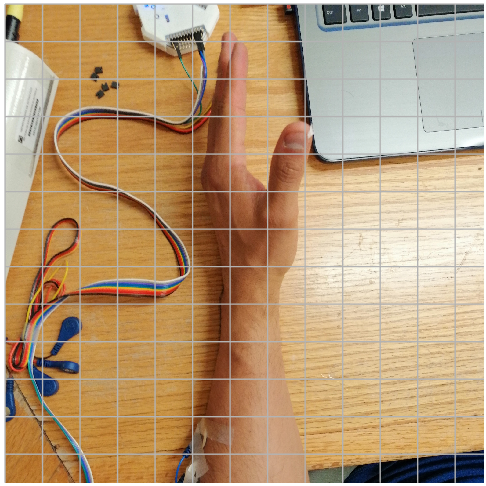
\includegraphics[width=\textwidth]{AI_g.png}
		\caption{}
		\label{Figura: AI}
	\end{subfigure}
%	\hfill
	\begin{subfigure}[htbp]{0.4\textwidth}
		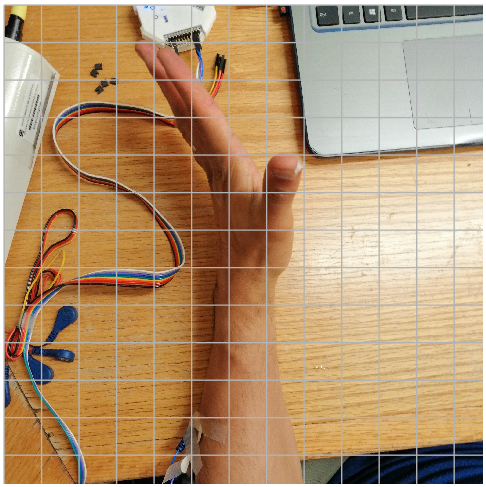
\includegraphics[width=\textwidth]{AC_g.png}
		\caption{}
		\label{Figura: AC}
	\end{subfigure}
%	\hfill
	\newline
	\begin{subfigure}[htbp]{0.4\textwidth}
		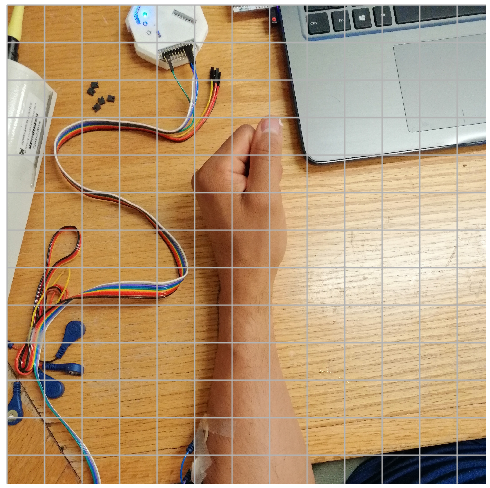
\includegraphics[width=\textwidth]{CI_g.png}
		\caption{}
		\label{Figura: CI}
	\end{subfigure}
%	\hfill
	\begin{subfigure}[htbp]{0.4\textwidth}
		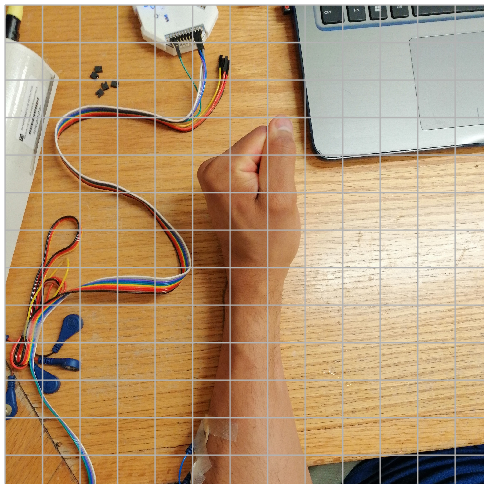
\includegraphics[width=\textwidth]{CC_g.png}
		\caption{}
		\label{Figura: CC}
	\end{subfigure}
%	\hfill
	\newline
	\begin{subfigure}[htbp]{0.4\textwidth}
		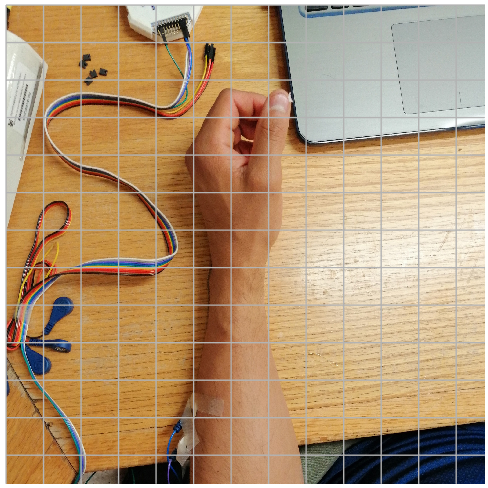
\includegraphics[width=\textwidth]{DD_g.png}
		\caption{}
		\label{Figura: DD}
	\end{subfigure}
	\caption[Posturas de mano para calibración de umbrales RMS]{Posturas de mano para calibración de umbrales RMS de los 5 movimientos. Se agregó una cuadrícula a la imagen para poder observar las diferencias entre las posturas. (a) Apertura incompleta (AI). (b) Apertura completa (AC). (c) Pinza gruesa incompleta (CI). (d) Pinza gruesa completa (CC). (e) Descanso (DD).}
	\label{Figura: Posturas}
\end{figure}

\newpage
\subsection{Validación fuera de línea}
El propósito de esta prueba consiste en obtener un indicador que proporcione información sobre el desempeño del sistema, al configurarlo con los parámetros obtenidos en la calibración, en su función de clasificación de movimientos.

%Para obtener dicho indicador, se diseñó un script en MATLAB\textregistered \; que lee el registro de sEMG crudo obtenido en la etapa de calibración, posteriormente le aplica una etapa de procesamiento (filtrado (descrito en la sección \ref{Sec: Procesamiento}), cálculo de RMS y suavizado) y por último se aplica el algoritmo de control diseñado (FSM y control proporcional). Una vez obtenida la salida del algoritmo de control, se procede a realizar el conteo de los errores y aciertos que tuvo el sistema al realizar la clasificación de los movimientos, expresando dichos valores en términos de porcentaje. Si el porcentaje obtenido de acierto es igual o mayor al 80$\%$ se acepta la calibración como exitosa y se procede a configurar el sistema diseñado en Simulink\textregistered \; con los parámetros arrojados en la calibración; en caso contrario, se revisa si existen problemas en la colocación de electrodos para registro de sEMG y se repite el proceso de calibración.

Para obtener dicho indicador se diseñó un script en MATLAB \textregistered \; el cual lleva a cabo el siguiente funcionamiento:

\begin{enumerate}
	\item Lectura de registro crudo de sEMG obtenido en etapa de calibración.
	\item Aplicación de etapa de procesamiento (filtrado (descrito en la sección \ref{Sec: Procesamiento}), cálculo de RMS y suavizado).
	\item Aplicación de algoritmo de control diseñado (FSM y control proporcional).
	\item Realizar conteo de aciertos y errores en la clasificación de movimientos.
	\item Mostrar valor de aciertos y errores en términos de porcentaje (Cuadro \ref{Cuadro:PorcentajesObtencion}).
\end{enumerate}

Una vez obtenido el porcentaje de aciertos y errores, se toma la decisión de aceptar o rechazar los parámetros obtenidos de la calibración. En caso de obtener un porcentaje mayor o igual al 80\% se aceptan los parámetros y se procede a configurar el sistema sEMG-FES diseñado en Simulink \textregistered \; con dichos parámetros. En caso contrario, se revisa la posibilidad de errores en la colocación de electrodos para registro de sEMG y se repite el proceso de calibración.

Cabe mencionar que los registros de calibración se conforman de dos repeticiones de la siguiente secuencia de movimientos:

\begin{enumerate}
	\item Descanso (DD): 9 segundos
	\item Cierre incompleto (CI): 3 segundos
	\item Cierre completo (CC): 6 segundos
	\item Cierre incompleto (CI): 3 segundos
	\item Descanso (DD): 9 segundos
	\item Apertura incompleta (AI): 3 segundos
	\item Apertura completa (AC): 6 segundos
	\item Apertura incompleta (AI): 3 segundos
\end{enumerate}

%Cuadro porcentajes aciertos y errores 
\begin{table}[htbp]
	\centering
	\begin{tabular}{|l|c|c|}
	\hline
	\textbf{Movimiento} & \textbf{Aciertos} & \textbf{Errores}\\ \hline \hline
	Apertura de mano & $\frac{Aciertos_{apertura}}{Aciertos_{apertura}+Errores_{apertura}}*100$ & $\frac{Errores_{apertura}}{Aciertos_{apertura}+Errores_{apertura}}*100$\\ \hline
	Descanso & $\frac{Aciertos_{descanso}}{Aciertos_{descanso}+Errores_{descanso}}*100$ & $\frac{Errores_{descanso}}{Aciertos_{descanso}+Errores_{descanso}}*100$\\ \hline
	Pinza gruesa & $\frac{Aciertos_{pinza}}{Aciertos_{pinza}+Errores_{pinza}}*100$ & $\frac{Errores_{pinza}}{Aciertos_{pinza}+Errores_{pinza}}*100$\\ \hline	
	\textbf{TOTAL} & $\frac{Aciertos_{totales}}{Aciertos_{totales}+Errores_{totales}}*100$ & $\frac{Errores_{totales}}{Aciertos_{totales}+Errores_{totales}}*100$\\ \hline
	\end{tabular}
	\caption{Matriz de confusión para prueba fuera de línea.}
	\label{Cuadro:PorcentajesObtencion}
\end{table}


%\newpage
\subsection{Validación en línea (control por biofeedback)}
%Una vez que el sistema se ha validado fuera de línea, se procede a realizar una prueba para corroborar su funcionamiento en línea. Para esto, se configura el bloque \emph{Control} del sistema completo implementado en Simulink\textregistered \; (Figura \ref{Figura: SisComp}) con los valores de los parámetros obtenidos en la calibración. Posteriormente, se configura el switch \emph{Habilitar estimulación} a ceros (para evitar la salida de estimulación real, pues en esta validación no se usa), y por último, se configura el tiempo de termino de la simulación a 60 s.

Una vez que el sistema se ha validado fuera de línea, se procede a realizar una prueba para corroborar su funcionamiento en línea. Para llevar a cabo esto se utiliza el sistema sEMG-FES implementado en Simulink\textregistered \; (Figura \ref{Figura: SisComp}) configurándolo de la siguiente manera:

\begin{enumerate}
	\item Se configura el bloque \emph{Control} con los valores de los parámetros obtenidos en la calibración.
	\item Se conecta el switch \emph{Habilitar estimulación} a \emph{Ceros} para evitar la salida de estimulación eléctrica real, pues en esta validación no se usa.
	\item Se configura el tiempo de término de la simulación con un valor de 60 s.
\end{enumerate}

%Sistema completo
\begin{figure}[htbp]
	\centering
	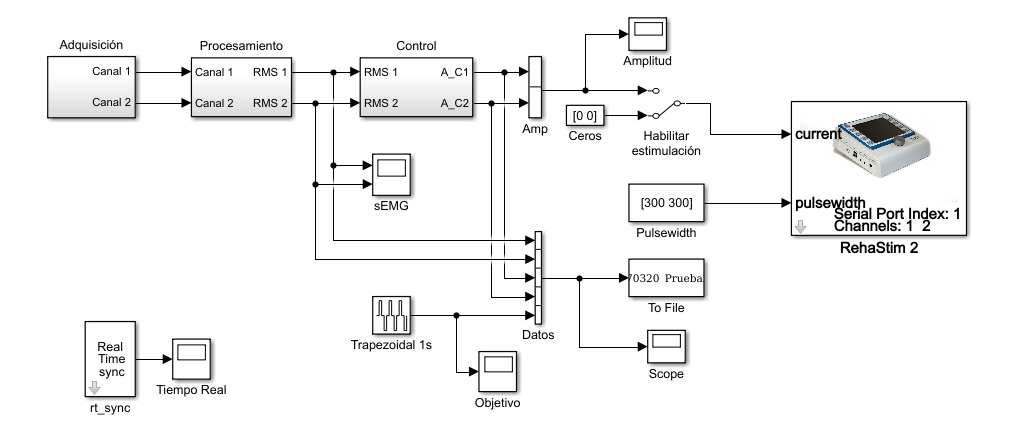
\includegraphics[width=\textwidth]{SistemaCompleto.png}
	\caption{Diagrama de bloques del sistema sEMG-FES implementado en Simulink\textregistered.}
	\label{Figura: SisComp}
\end{figure}

\newpage
Posteriormente, se le indica al sujeto la forma en la que se llevará a cabo la prueba y cómo deberá realizarla. Para esto, al sujeto se le mostrará en un scope una señal trapezoidal con ciclos negativos y ciclos positivos (Figura \ref{Figura: Trapezoidal}), el sujeto deberá realizar el seguimiento de dicha trapezoidal considerando que el ciclo positivo indica apertura de mano completa, mientras que el ciclo negativo indica pinza gruesa completa y que una línea en cero indica descanso. El sujeto deberá realizar una transición suave y continua entre los movimientos indicados buscando seguir visualmente las pendientes de la trapezoidal. Una vez dadas las indicaciones se procede a iniciar la prueba, y a la par el experimentador deberá observar en otro scope la salida del bloque de control, donde se observará si la activación de canales de estimulación eléctrica corresponden a los movimientos que realiza el sujeto. La detección de un movimiento de pinza gruesa activa el canal 1 de estimulación, y la detección del movimientos de apertura de mano activa el canal 2 de estimulación.
% (pinza gruesa activa canal 1 de estimulación, apertura de mano activa canal 2 de estimulación, y descanso no activa algún canal de estimulación).

\vfill
%Trapezoidal
\begin{figure}[htbp]
	\centering
	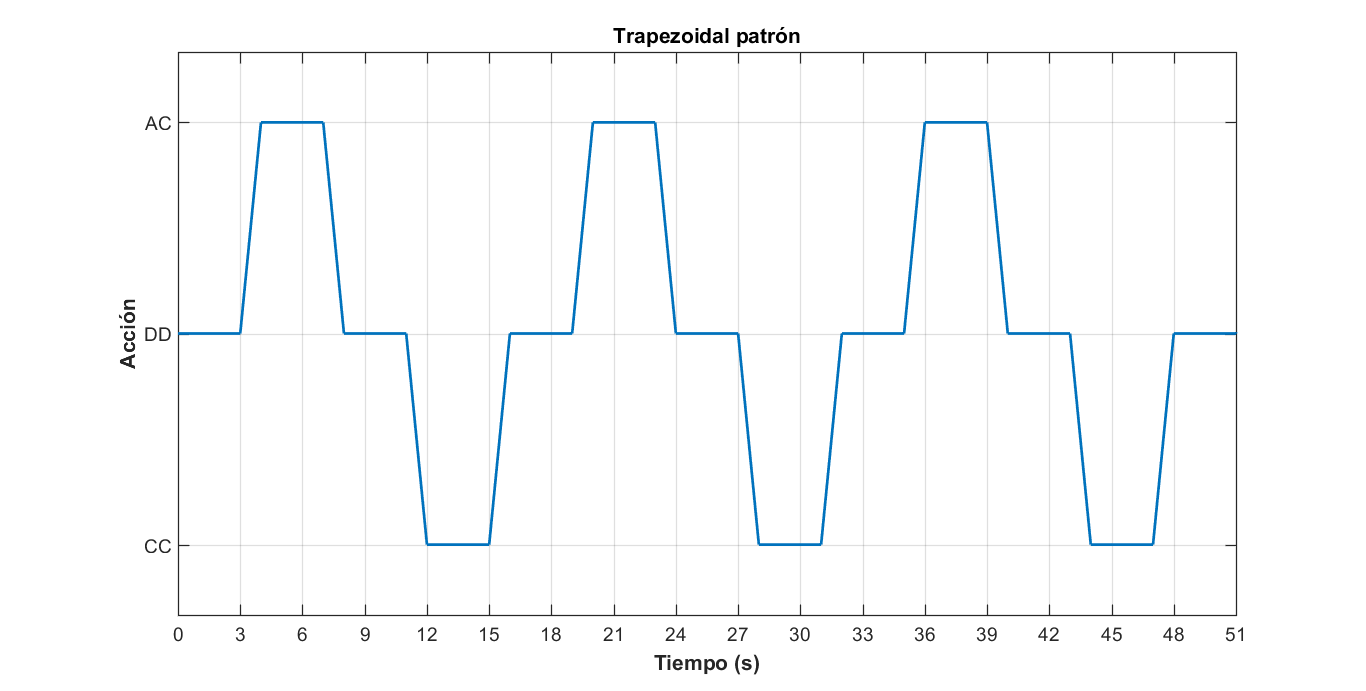
\includegraphics[width=\textwidth]{Trapezoidal.png}
	\caption[Segmento de señal trapezoidal patrón]{Segmento de señal trapezoidal utilizada como guía visual para el sujeto en la prueba en línea. El ciclo positivo indica al sujeto que realice un movimiento de apertura completa (AC), el ciclo negativo indica al sujeto que realice un movimiento de pinza gruesa completa (CC), mientras que el valor en cero indica que realice un descanso (DD).}
	\label{Figura: Trapezoidal}
\end{figure}
\vfill

\newpage
\subsection{Tarea funcional síncrona}\label{Sec: TareaObj}
En esta prueba final se utilizan los mismos parámetros e indicaciones que en la prueba de validación en línea, sin embargo, para esta prueba se aplica estimulación eléctrica al brazo afectado del sujeto, por lo que el switch \emph{Habilitar estimulación} se encuentra conectado la salida del bloque \emph{Control}, y además, el tiempo de término de la simulación se configura a 180 s.

En esta prueba se mide el tiempo de retardo que existe entre el inicio del movimiento en la mano ``sana'' (generado de manera voluntaria) y el inicio del movimiento en la mano afectada (generado por FES). Para poder realizar esto se almacenan todos los datos de las señales involucradas en el sistema (registros de sEMG, patrones de estimulación eléctrica y señal trapezoidal patrón), y posterior a la finalización de la prueba se realiza un análisis manual en MATLAB\textregistered \; donde se determina el tiempo de retardo existente para cada movimiento, y se obtiene el promedio del retardo de todas las repeticiones realizadas para obtener un retardo global de la sesión.

\subsection{Tarea funcional asíncrona}\label{Sec: TareaFunAsin}
%Se diseñó una tarea de tiempo libre donde pudiera demostrarse la utilidad del sistema diseñado para realizar alguna tarea funcional útil para el sujeto, que consistió en el agarre de un objeto, su traslado y liberación. Para ello, configurando el sistema sEMG-FES de la misma forma en la cual se configuró para la tarea funcional síncrona, cambiando en Simulink \textregistered \; el tiempo de término de la simulación a \emph{inf}. Sobre la mesa donde descansan los antebrazos y manos del sujeto, se colocan dos objetos cilíndricos a unos cms de sus manos. Se le solicitó que con el miembro sano fuera tomando dicho objeto, mientras que con ayuda de su hombro del miembro afectado fuera acercando su mano al otro objeto para, por efecto de la estimulación eléctrica, lograr tomarlo. Una vez que lograse tomarlo, con la misma ayuda de su hombro tendría que levantar dicho objeto y desplazarlo a un lugar diferente del lugar donde lo tomó y bajar suavemente dicho objeto para finalmente soltarlo. La Figura \ref{Figura: TareaFuncional_P} esquematiza los pasos de los que consta la tarea funcional asíncrona.

Se diseñó una prueba de tiempo libre donde pudiera demostrarse la utilidad del sistema diseñado para realizar alguna tarea funcional útil para el sujeto. Para esta prueba se configuró el sistema sEMG-FES de la misma forma en la cual se configuró dicho sistema para la realización de la tarea funcional síncrona, pero con un cambio en el tiempo de término de la simulación en Simulink \textregistered . Para esta prueba los antebrazos y manos del sujeto descansan sobre una mesa, en la cual se colocan dos objetos cilíndricos a unos centímetros de sus manos (un objeto en cada mano). Una vez configurado el sistema sEMG-FES y colocado el sujeto en la posición adecuada, se procede a llevar a cabo la tarea funcional asíncrona, la cual se describe en el Cuadro \ref{Cuadro:TareaFunAsin}, donde se describe el movimiento voluntario que deberá realizar el sujeto, el canal de sEMG que debería presentar mayor actividad, el canal FES que debería activar dicho movimiento, el movimiento generado por FES que se espera, y la correspondencia de dicho movimiento con su representación gráfica en la Figura \ref{Figura: TareaFuncional_P}.

Cabe mencionar que desde los incisos (c) al (e) del Cuadro \ref{Cuadro:TareaFunAsin} , el sujeto debe mantener sostenido el movimiento voluntario de pinza gruesa en la mano izquierda, y se espera esto genere la estimulación eléctrica necesaria para sostener el objeto con la mano derecha, esto sin realizar algún esfuerzo voluntario en dicha mano.

%Cuadro descriptivo de tarea funcional
\begin{table}[htbp]
	\centering
	\begin{tabular}{|p{5cm}|p{1.4cm}|p{1.4cm}|p{3.5cm}|p{1.5cm}|}
	\hline
	\textbf{Movimiento voluntario} & \textbf{Canal sEMG activo} & \textbf{Canal FES activo} & \textbf{Movimiento FES} & \textbf{Figura}\\ \hline \hline
	Abducción del hombro en ambos brazos para acercar mano a objeto cilíndrico cercano. & Nulo. & Nulo. & Ninguno. & Figura \ref{Figura: TareaFuncional_P}(a)\\ \hline
	Extensión de dedos con mano ``sana'' (izquierda). En ambos brazos se deberá acercar la palma abierta al correspondiente objeto. & 2 & 2 & Apertura de mano ``afectada'' (derecha). & Figura \ref{Figura: TareaFuncional_P}(b)\\ \hline
	Flexión de dedos con mano "sana" (izquierda) para lograr tomar el objeto. & 1 & 1 & Pinza gruesa en mano ``afectada'' (derecha) para tomar objeto. & Figura \ref{Figura: TareaFuncional_P}(c)\\ \hline
	Abducción y extensión de ambos hombros para levantar objetos 10 cm de la mesa y trasladarlos lateralmente 10 cm de su posición original. & 1 & 1 & Pinza gruesa en mano ``afectada'' (derecha) & Figura \ref{Figura: TareaFuncional_P}(d)\\ \hline
	Flexión de ambos hombros para bajar objetos a la altura de la mensa. & 1 & 1 & Pinza gruesa en mano ``afectada'' (derecha) & Figura \ref{Figura: TareaFuncional_P}(e)\\ \hline
	Extensión de dedos con mano ``sana'' (izquierda) para soltar objeto sobre la mesa. & 2 & 2 & Apertura de mano ``afectada'' (derecha) para soltar objeto sobre la mesa. & Figura \ref{Figura: TareaFuncional_P}(f)\\ \hline
	\end{tabular}
	\caption{Descripción detallada de tarea funcional asíncrona.}
	\label{Cuadro:TareaFunAsin}
\end{table}

%Figura tarea funcional (manitas)
\begin{figure}[htbp]
	\centering
	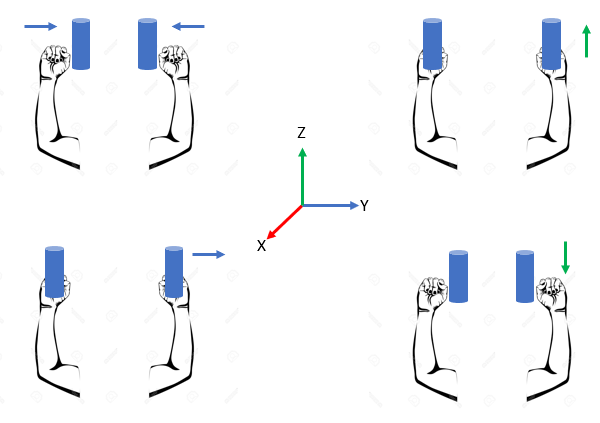
\includegraphics[width=\textwidth]{TareaFuncional.png}
	\caption[Esquema de tarea funcional con tiempo libre.]{Esquema de tarea funcional con tiempo libre. Las flechas indican el movimiento que de se deberá realizar con ayuda de los hombros: Flecha azul (eje Y) representa movimientos horizontales; Flecha roja (eje X) representa movimientos verticales; Flecha verde (eje Z) representa movimientos hacia arriba y abajo. Cada inciso corresponde a un movimiento descrito en el Cuadro \ref{Cuadro:TareaFunAsin}.}
	\label{Figura: TareaFuncional_P}
\end{figure}


%Se diseñó un sistema basado en una combinación de máquina de estados finitos con un control lineal. El sistema requiere de un proceso de calibración previa donde se obtienen 8 umbrales tras la repetición de 4 movimientos, dos umbrales corresponden a los valores RMS promedio de los dos canales de adquisición a lo largo de la tarea \emph{cierre de mano ligero}, otros dos corresponden a los valores RMS promedio de la tarea \emph{cierre de mano completo}, mientras que los 4 restantes corresponden a los valores RMS promedio de las tareas \emph{apertura de mano ligera} y \emph{apertura de mano completa}. Además, tras la calibración se obtiene también un factor denominado \emph{detector de movimiento}, el cual se obtiene tras calcular la diferencia promedio entre los canales de adquisición a lo largo de la tarea de apertura de mano. Adicionalmente se realiza una calibración de la estimulación eléctrica, la cual utiliza el sistema de colocación de electrodos de estimulación descrito en \cite{AnaMartin2019}, donde se obtiene los valores en amplitud de los umbrales motores y funcionales de las tareas de apertura y cierre de mano.
%
%El detector de movimiento se utiliza para realizar el control por máquina de estados finitos (Figura \ref{Figura: FSM_Control}), la cual consisten en determinar si la diferencia de amplitudes entre canales ha pasado el valor del detector de movimiento, si es así, el control prosigue con la tarea de apertura de mano, en caso contrario, el control procede a la tarea de cierre de mano.
%
%\begin{figure}[htbp]
%	\centering
%	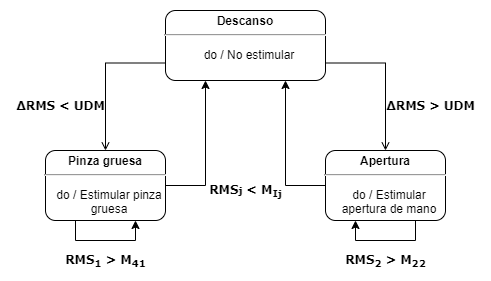
\includegraphics[scale=0.9]{FSM_Control.png}
%	\caption[FSM para control]{Máquina de estados finitos encargada de la detección de movimiento e inicio del control lineal.}
%	\label{Figura: FSM_Control}
%\end{figure}
%
%Dentro del control de cada tarea, se utilizan los umbrales de las tareas ligeras para realizar la activación del control lineal, el cual modula la amplitud de la corriente eléctrica, del canal asociado al movimiento detectado, utilizando la recta descrita por la Ecuación \ref{Ecu: Mapeo}, donde $A$ representa la amplitud que inyectará el estimulador eléctrico, $A_{max}$ es el umbral funcional de estimulación eléctica, $A_{min}$ es el umbral motor de estimulación eléctica, $D$ representa el valor RMS actual, mientras que $D_{max}$ y $D_{min}$ representan los umbrales RMS de la tarea completa y ligera del canal asociado al movimiento detectado (canal 1 para cierre de mano y canal 2 para apertura de mano). Adicionalmente se aplica la función máximo entero a la recta debido a que el dispositivo de estimulación eléctrica sólo admite valores enteros, y también se aplica un criterio de saturación de corriente eléctrica para evitar que tras una contracción muscular muy fuerte se genere un valor de amplitud de corriente eléctrica dañino para el sujeto.
%
%%Ecuación mapeo lineal
%\begin{equation}
%	A = \frac{A_{max} - A_{min}}{D_{max} - D_{min}}(D - D_{min}) + A_{min}
%	\label{Ecu: Mapeo}
%\end{equation}

%\section{Tarea objetivo}
%{\color{red}INCLUIR TAREA OBJETIVO DE ENTRENAMIENTO CON TRAPEZOIDAL EN LÍNEA}
